
A simple analytical turbine model is presented to describe the interaction between blade pitching, flapwise tip deflection, flapwise root bending moment and all external disturbances. The model uses observations in section XX (the above section), and is presented in a way to guide the design of a controller.


\section{Background}



A block diagram of a wind turbine system without IPC is presented in Figure \ref{fig:analModel:1}. The tip deflection of the $ith$ blade, $x_i$, is considered an output of this system. The two relevant inputs for system are the blade pitch angle, $\theta_i$, and all other disturbances which influence tip deflection, which is encapsulated in the input term $d(t)$. $d(t)$ represents disturbances from wind shear, tower shadow, yaw misalignment and turbulence. Although it may seem oversimplistic to encapsulate these disturbances into a single signal, it is clear from Figure \ref{fig:??} that the majority of the energy of this disturbance is concentrated at $f_{1P}$. The collective pitch control loop is presented in this figure to show how a typical wind turbine controls pitch angle to achieve a desired power output. 


Figure \ref{fig:analModel:1} is augmented in Figure \ref{fig:analModel:2} to include IPC action. Whereas the collective pitch control responds to changing rotor speed, the collective pitch control responds to the tip deflection of all three blades. Note how the total pitch demand is a superposition of the collective and individual pitch control loops. This control architecture is common in literature (see XXXXX), and is justified by the fact that the bandwidth of the CPC is much lower than the IPC loops. To demonstrate this, see Figure (something in results section)). 

\myFigure{Turbine_blockdiagram_IPC.png}{cap}{fig:analModel:2}

Due to the highly nonlinear nature of the wind turbine system, the models presented in literature vary greatly. It is found in this project that a linear approximation of the turbine system is adequate in designing a controller that provides load reductions using tip deflection inputs. This assumption is supported in literature for IPC systems using strain gauge sensors (see bossanyi, Lu, XX). By encapsulating and linearising the wind turbine model as well as the CPC loop about a fixed rotor speed, tip deflection and blade pitch angle, $\overline{\Omega}$, $\overline{x}$, $\overline{\theta}$ respectively, the block diagram can be split into a plant block, $P(s)$ and a controller block, $K(s)$, with a disturbance input, $d(s)$, and tip deflection of each blade in the vector $\tilde{x}(s)$. Note an additional assumption is put in place in this block diagram. Namely, the disturbance signal and pitch demand signal are additive. Therefore, the effect of any disturbance signal can be rejected by providing an appropriate pitch demand signal. 
\myFigure{Turbine_blockDiagram_P_K.png}{cap}{fig:analModel:3}

The total system is simplified to a single linear block in Figure \ref{fig:analModel:4}. The transfer function between the disturbances and the tip deflection output now match the disturbance rejection model outlined in section XX. In order to use this model to design a controller, the plant, $P$, shall be estimated using system identification.
\myFigure{Turbine_blockDiagram_supersimple.png}{cap}{fig:analModel:4}

\section{System Identification of Plant}
The design of the controller transfer function is dependant on the wind turbine system (plant). The plant for the purpose of this project is a SISO transfer function between blade pitch angle (the input), and blade tip deflection (the output). To find the transfer function which best describes the relationship between the input and output signal, system identification  is performed. In particular, the magnitude and phase response of the blade system is of interest as this will be used to shape the controller loop. 
\\~\\
System identification is the act of estimating the system dynamics of a blackbox system without prior knowledge of the system. One method of performing system identification is to perform a frequency sweep. A frequency sweep involves subjecting the blackbox system to a sinusoidal input of a particular frequency, and measuring the amplitude and phase response of the output signal. This is repeated for a range of frequencies to estimate the frequency response of the system, from which a transfer function can be fitted. A more efficient way of performing system identification is to subject the system to the a step input and to fit a transfer function to the step response of the system. Theoretically, this is valid because a step signal is composed of a wide range frequencies, and is therefore typically used in system identification problems \citep{19_ljung1998system}. Using the System Identification Toolbox in Matlab, the transfer function of a system can be estimated given an arbitrary input signal and its corresponding output signal.
\\~\\
The task at hand is as follows. An unknown system, $G$, is subjected to an input $x(t)$ and has a corresponding output $y(t)$. Given $x(t)$ and $y(t)$, find an LTI system $\tilde{G}$ which approximates the frequency response characteristics of $G$.
\\~\\
This task is applied using the DTU10MW turbine in HAWC2 as the unknown system, the pitch demand of one blade as the input signal, and the flapwise tip deflection as an output. The stiff turbine model is used in HAWC2 to generate the system output in order to isolate the effects of pitching on flapwise tip deflection. At 120 seconds and XX seconds, a step input is provided to one of the blade pitch actuators. The resultant tip deflection time series is measured. It is assumed that the behaviour of the blade system depends on the turbine operating conditions (rotor speed, pitch angle), and therefore different transfer functions are found over a range of wind speeds, $U = 4, 6, ..., 26 m/s$. 
 
Figure \ref{fig:pitchstep_18} shows time series data from the HAWC2 simulations used for the system identification at a wind speed of $18m/s$. The tip deflection can be seen to respond only to the step changes in pitch angle, and converge to a constant value at all other times, verifying the simulation is not influenced by other aerodynamic and structural influences. To verify (validate?) the linearity assumption of the system, two steps are provided at different amplitudes. From the figure it can be seen that at above rated wind speed, the step size of the output signal scales with the magnitude of the input step, which supports the underlying assumption that the blade system behaves linearly under small pitch perturbations. Below rated wind speed, this linearity does not hold as well as can be seen in Table \ref{tab:linearity}. This is likely a result of the long length of the step, during which, the rotor speed changes which has the effect of changing the thrust and therefore the tip deflection. 

\myFigure{pitchstep_18.png}{cap}{fig:pitchstep_18}
Figure \ref{fig:Blade_TF18} shows the bode plot corresponding to the time series data in \ref{fig:pitchstep_18}. The blue line shows a frequency response estimation using MATLABs \texttt{spafdr} function, and the orange line is the transfer function fit using MATLABs \texttt{tfest} function. 
\myFigure{Blade_TF_18.png}{cap}{fig:Blade_TF18}

%figuers made in modelling/preproc....py
\begin{figure}[H]
        \centering
        \begin{subfigure}[b]{0.48\textwidth}
            \centering
            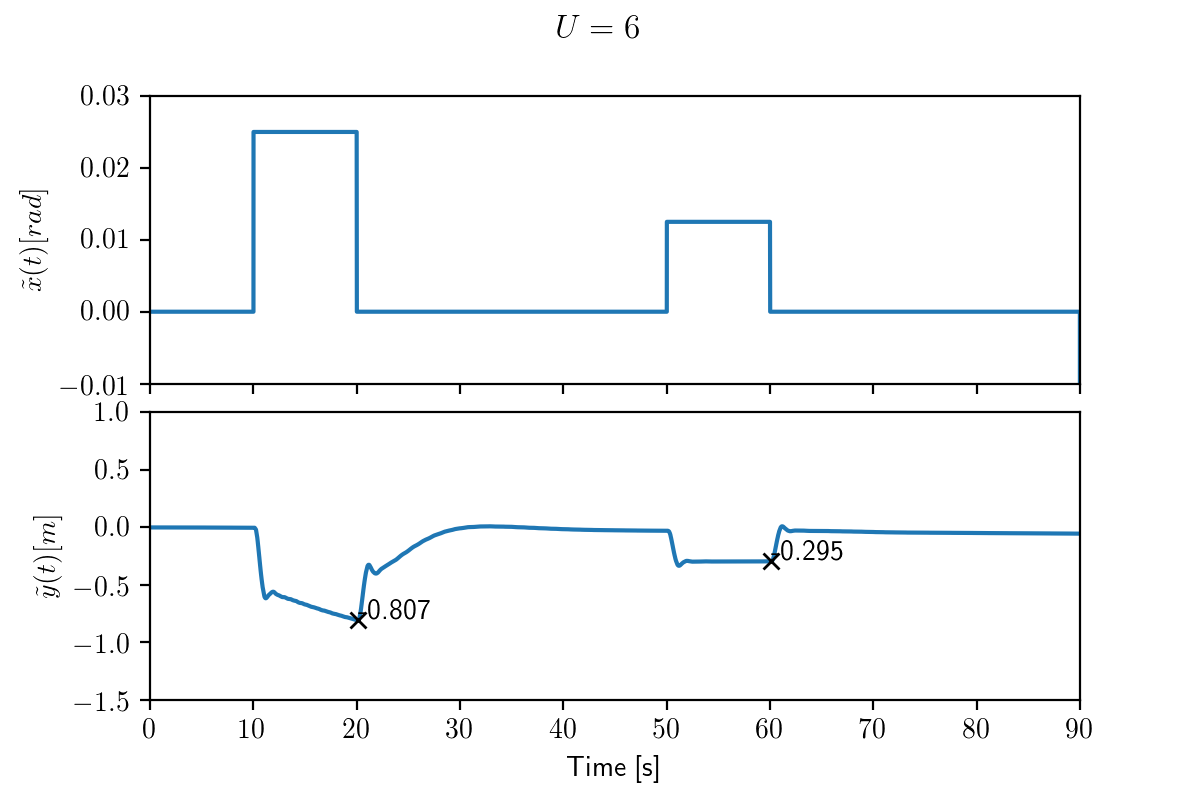
\includegraphics[width=\textwidth]{pitchstep_6.png}
            \caption[Network2]%
            {{\small a}}    
            \label{fig:mean and std of net14}
        \end{subfigure}
        \hfill
        \begin{subfigure}[b]{0.48\textwidth}  
            \centering 
            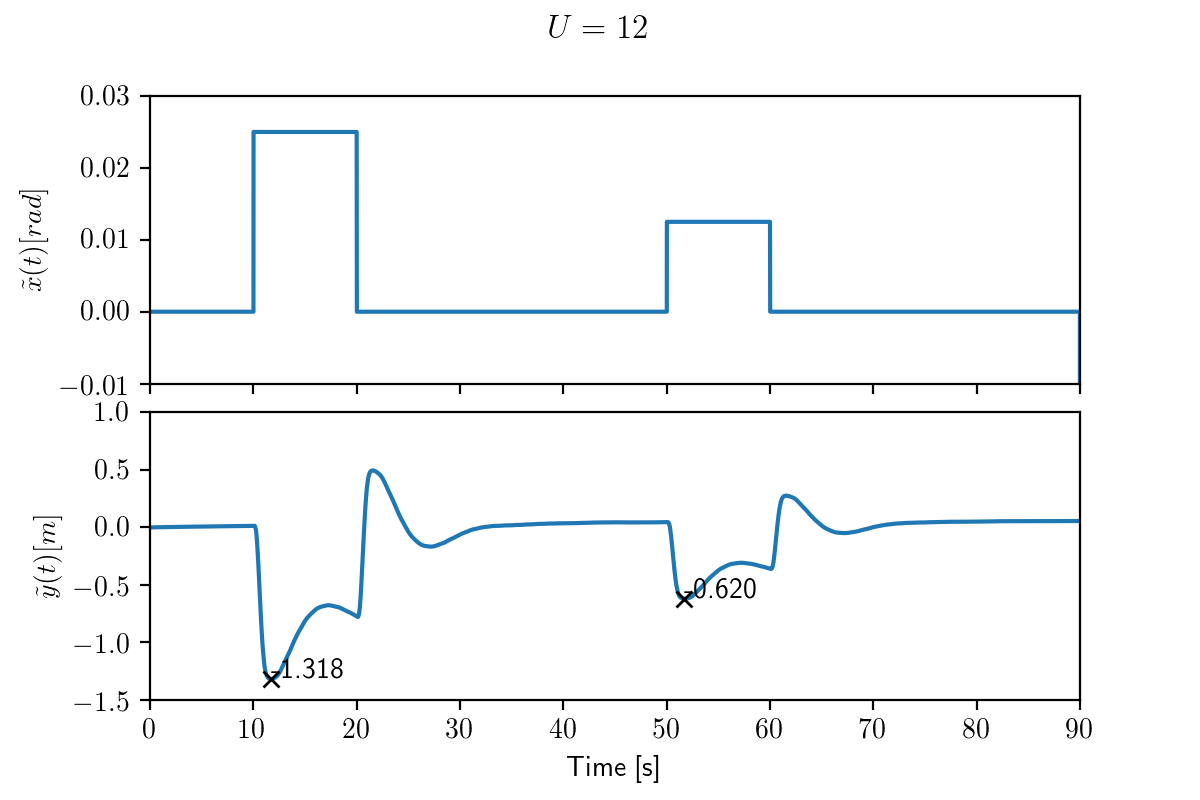
\includegraphics[width=\textwidth]{pitchstep_12.png}
            \caption[]%
            {{\small a}}    
            \label{fig:mean and std of net24}
        \end{subfigure}
        \vskip\baselineskip
        \begin{subfigure}[b]{0.48\textwidth}   
            \centering 
            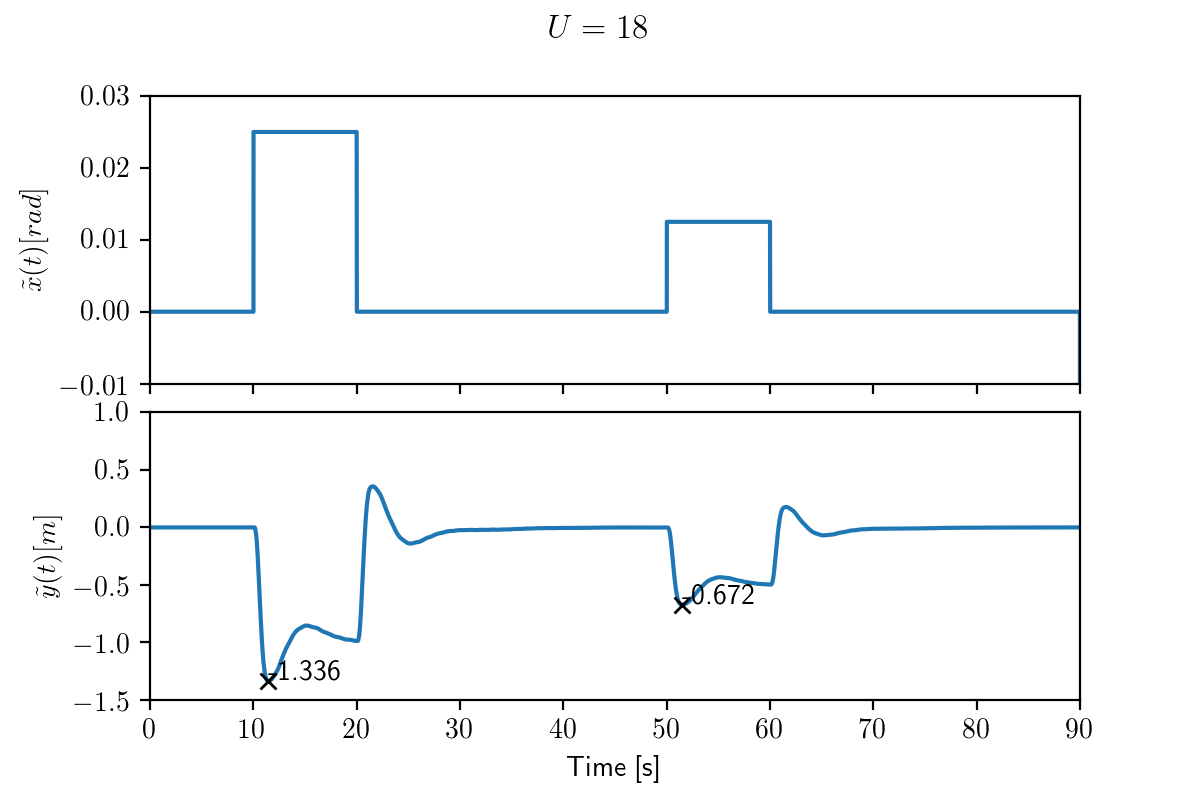
\includegraphics[width=\textwidth]{pitchstep_18.png}
            \caption[]%
            {{\small a}}    
            \label{fig:mean and std of net34}
        \end{subfigure}
        \quad
        \begin{subfigure}[b]{0.48\textwidth}   
            \centering 
            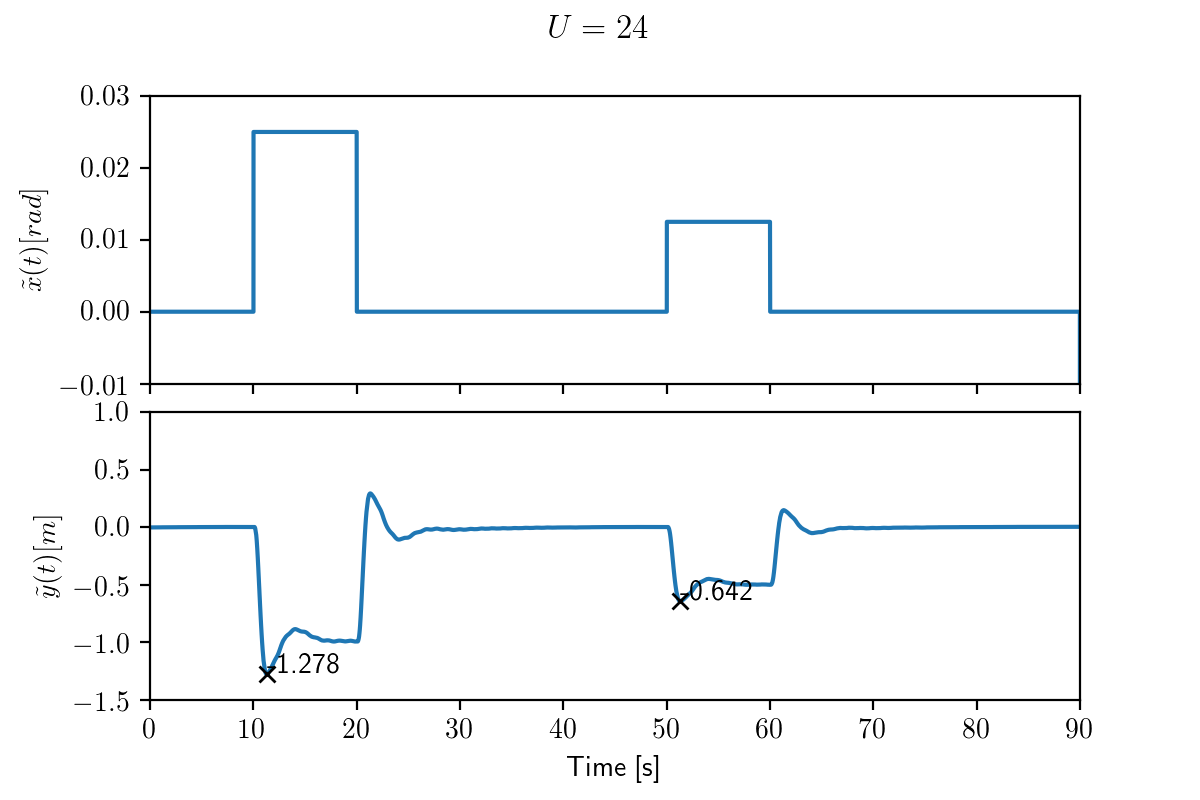
\includegraphics[width=\textwidth]{pitchstep_24.png}
            \caption[]%
            {{\small a}}    
            \label{fig:mean and std of net44}
        \end{subfigure}
        \caption[adsf ]
        {\small asdf} 
        \label{fig:mean and std of nets}
    \end{figure}
    
    
    
    
    
\begin{table}[]
\centering
\caption{My caption}
\label{tab:linearity}
\begin{tabular}{c|ccc}
Windspeed [m/s] & $y_1$  & $y_2$ & $y_1/y_2$ \\ 
\hline
4 & -0.782 & -0.485 & 1.612 \\
6 & -0.807 & -0.295 & 2.736 \\
8 & -0.892 & -0.597 & 1.494 \\
10 & -1.162 & -0.726 & 1.600 \\
12 & -1.318 & -0.620 & 2.127 \\
14 & -1.368 & -0.698 & 1.960 \\
16 & -1.358 & -0.685 & 1.983 \\
18 & -1.336 & -0.672 & 1.987 \\
20 & -1.315 & -0.661 & 1.988 \\
22 & -1.295 & -0.651 & 1.988 \\
24 & -1.278 & -0.642 & 1.990 \\
26 & -1.259 & -0.632 & 1.993 \\
\end{tabular}
\end{table}

\section{Open Loop Output Estimation}
Now that $P$ has been estimated, the spectrum of the open loop output signal is required to be able to design the controller. The open loop output spectrum refers to the frequency decomposition of the flapwise tip deflection for a turbine without tip deflection control. This can be found by running simulations using the DTU10MW turbine with full structural flexibility, realistic aerodynamic effects including wind shear, tower shadow and turbulence. As with the plant model, it is assumed that the output spectrum is a function of operating conditions, and therefore a different spectrum is produced for each wind speed. 3 simulations of 10 minutes each with different turbulent seeds were run for each windspeed. From these simulations, time series data of tip deflection is collected for a particular blade, $i$, for each seed number, $j$, for each wind speed, $U$. For a given wind speed, The tip deflection spectrum, $Y_U(s)$ is by averaging the one sided discrete Fourier transformations, $\mathcal{F}$ for each blade in each seed. That is,

$$Y_U(\omega) = \frac{1}{3N_s}\sum^{3}_{i=1}\sum^{N_s}_{j=1}Y_{U,i,j}(\omega)$$
where the one sided Fourier transform is defined and normalized as:
$$Y_{U,i,j}(\omega)\xleftarrow{\mathcal{F}} \frac{2}{N}\sum^{(N-1)/2}_{n=0}y_{U,i,j}(t) \cdot e^{-n\frac{\omega i}{N}}$$

This particular normalization is chosen so that the frequency component amplitude matches the tip deflection amplitude in meters. In addition to averaging the spectrum over seeds and blades, the spectrum is smoothed by splitting each time series into segments with 256 data points each and taking the average of each of their spectra. Spectra for wind speeds of 6, 12, 18 and 14 $m/s$ are shown in on a log-log plot in Figure \ref{fig:Spectra_OL}. 

\begin{figure}[H]
        \centering
        \begin{subfigure}[b]{0.48\textwidth}
            \centering
            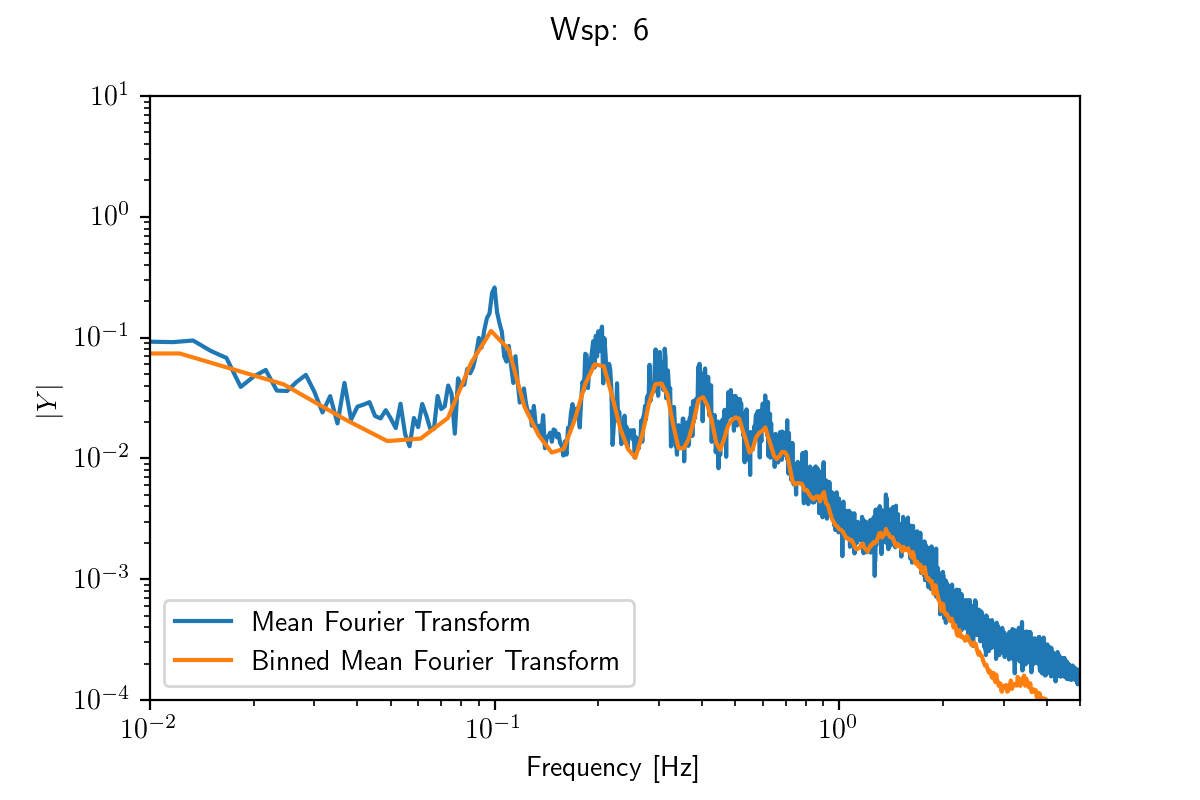
\includegraphics[width=\textwidth]{OLResponse_6.png}
            \caption[Network2]%
            {{\small a}}    
            \label{fig:mean and std of net14}
        \end{subfigure}
        \hfill
        \begin{subfigure}[b]{0.48\textwidth}  
            \centering 
            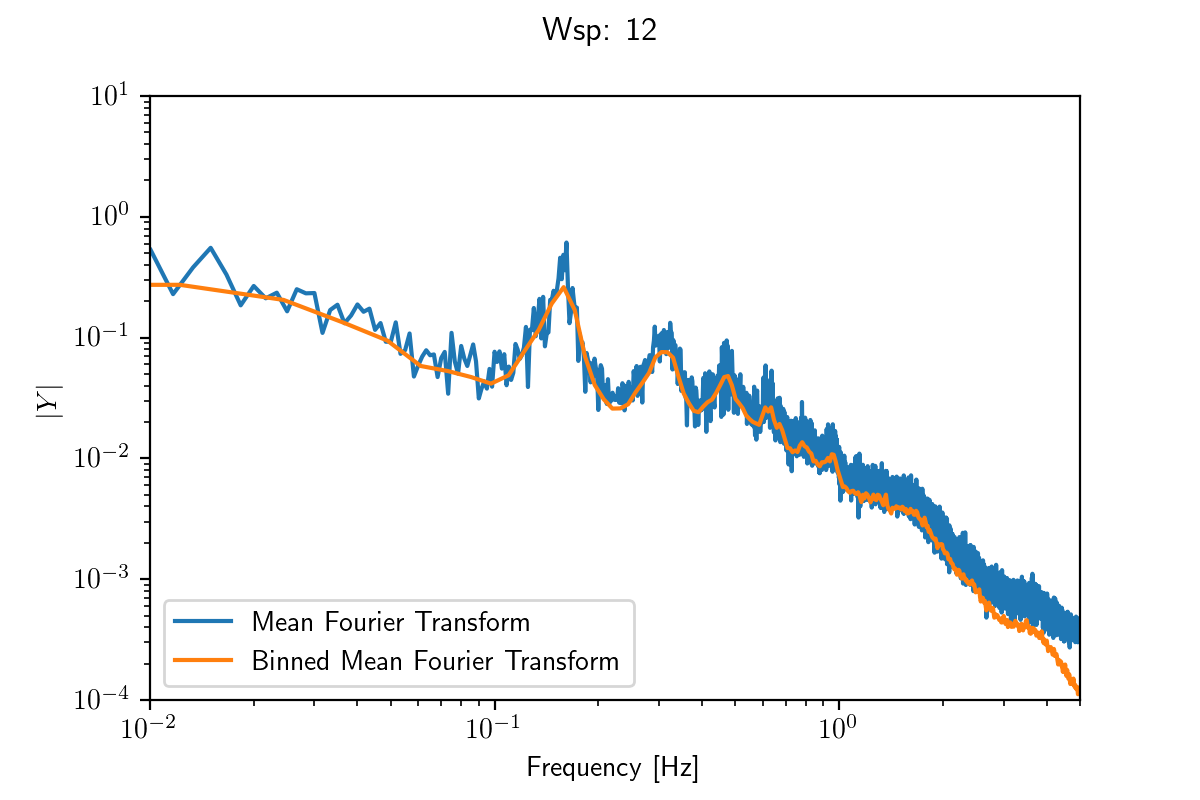
\includegraphics[width=\textwidth]{OLResponse_12.png}
            \caption[]%
            {{\small a}}    
            \label{fig:mean and std of net24}
        \end{subfigure}
        \vskip\baselineskip
        \begin{subfigure}[b]{0.48\textwidth}   
            \centering 
            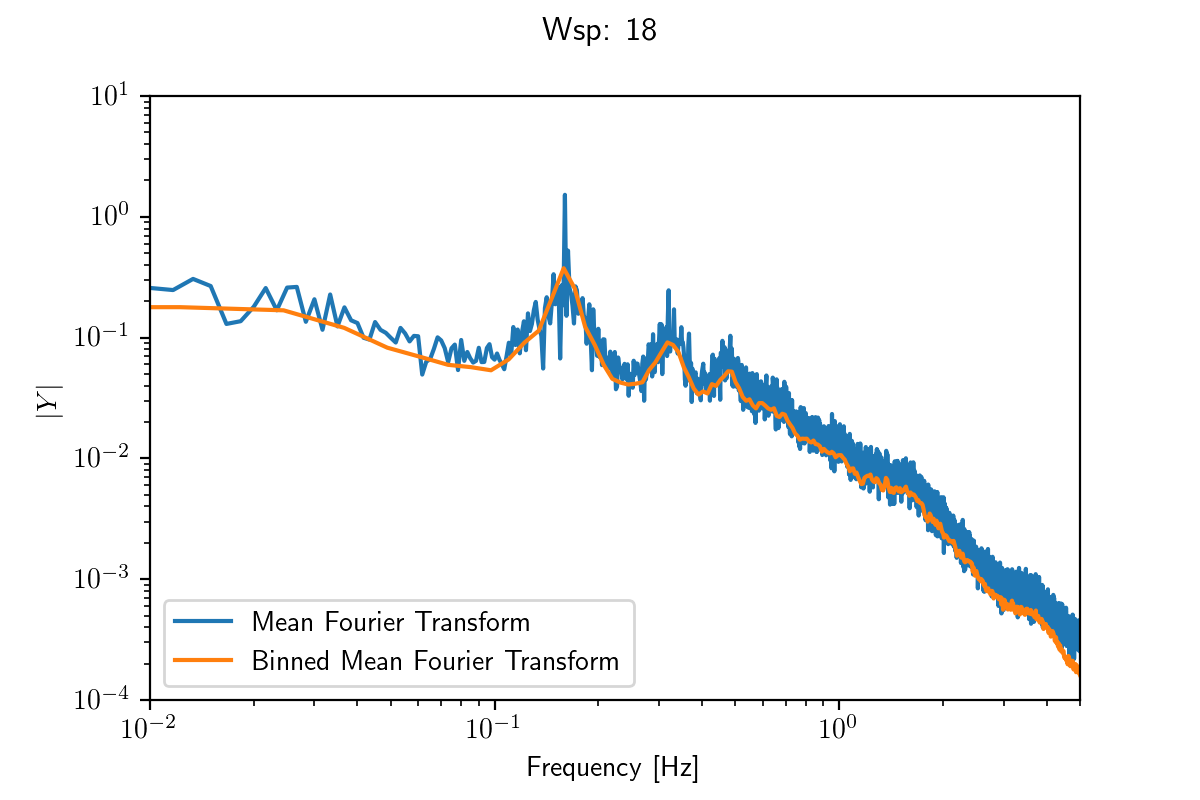
\includegraphics[width=\textwidth]{OLResponse_18.png}
            \caption[]%
            {{\small a}}    
            \label{fig:mean and std of net34}
        \end{subfigure}
        \quad
        \begin{subfigure}[b]{0.48\textwidth}   
            \centering 
            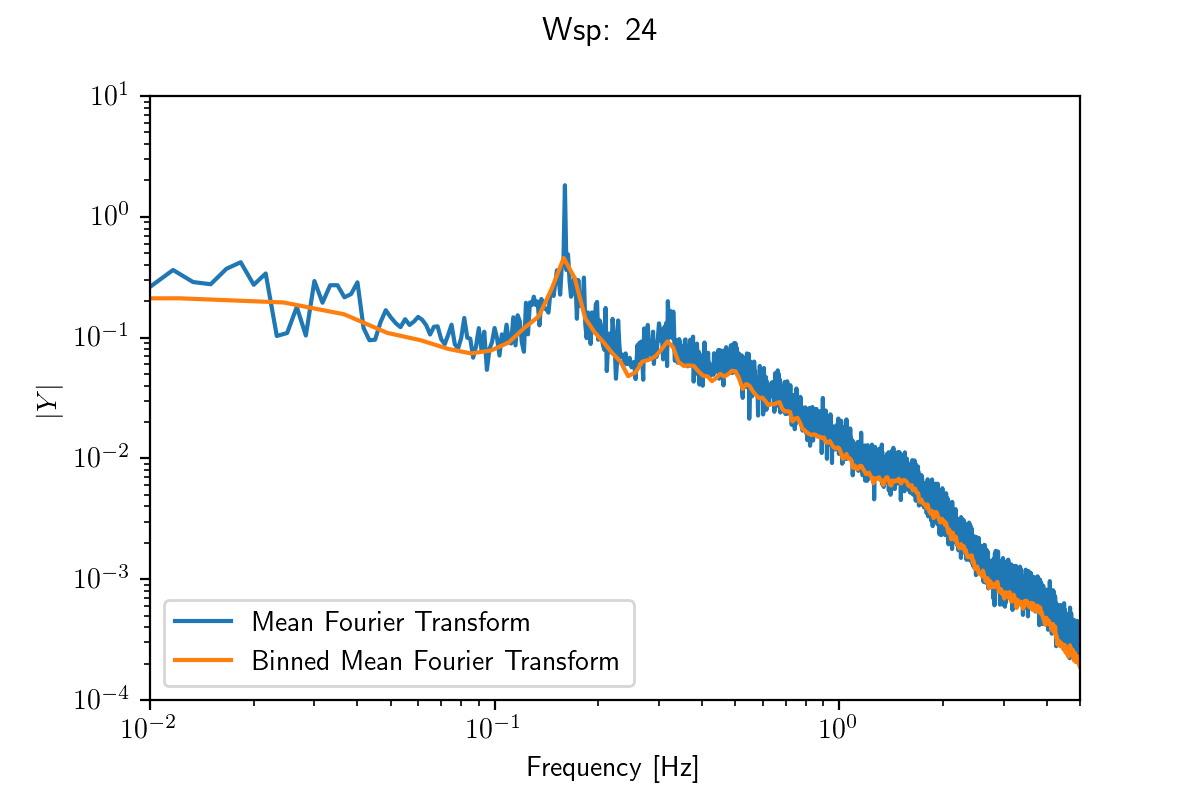
\includegraphics[width=\textwidth]{OLResponse_24.png}
            \caption[]%
            {{\small a}}    
            \label{fig:mean and std of net44}
        \end{subfigure}
        \caption[adsf ]
        {\small asdf} 
        \label{fig:Spectra_OL}
    \end{figure}